\section{Numerical Results and Discussion}
A laminate composite with dimensions $1000 \times 1000 \times 0.165 mm^3$ for
each lamina is under various loading cases, and each CA, GF, and GL layer is
assumed to cost 8, 2.5 and 1 monetary units, respectively. The other
material properties are shown in Table \ref{tab:mat}. A carbon/epoxy ply is represented by "cr", a
graphite/epoxy ply by "gl", and a glass/epoxy ply by "gl".  In the present
experiment, the optimal composite system, layup, thickness, and number of
layers for a targeted strength ratio (2 in this paper) under two different
in-plane loading conditions is investigated.

\begin{table*}[ht]
\caption{Comparison of the carbon/epoxy, graphite/epoxy, and glass/epoxy properties}
\centering
\begin{adjustbox}{width=1\textwidth}
\label{tab:mat}
\begin{tabular}{cccccc}
\toprule
Property								   & Symbol				  & Unit  &  Carbon/Epoxy&  Graphite/Epoxy  &  Glass/Epoxy   \\
\midrule
Longitudinal elastic modulus			   & $E_1$				  & GPa   &  116.6       &  181             &  38.6           \\
Traverse elastic modulus				   & $E_2$				  & GPa   &  7.67        &  10.3            &  8.27           \\
Major Poisson's ratio					   & $v_{12}$			  &       &  0.27        &  0.28            &  0.26           \\
Shear modulus							   & $G_{12}$			  & GPa   &  4.17        &  7.17            &  4.14           \\
Ultimate longitudinal tensile strength     & $(\sigma_1^T)_{ult}$ & MP    &  2062        &  1500            &  1062            \\
Ultimate longitudinal compressive strength & $(\sigma_1^C)_{ult}$ & MP    &  1701        &  1500            &  610             \\
Ultimate transverse tensile strength       & $(\sigma_2^T)_{ult}$ & MPa   &  70          &  40              &  31              \\
Ultimate transverse compressive strength   & $(\sigma_2^C)_{ult}$ & MPa   &  240         &  246             &  118              \\
Ultimate in-plane shear strength           & $(\tau_{12})_{ult}$  & MPa   &  105         &  68              &  72               \\
Density                                    & $\rho$               & $g/cm^3$ &  1.605    &  1.590           &  1.903               \\
Cost                                       &                      &       &  8           &  2.5             &  1               \\
\bottomrule
\end{tabular}
\end{adjustbox}
\end{table*}

%\begin{figure*}[!htb]
%	\centering
%	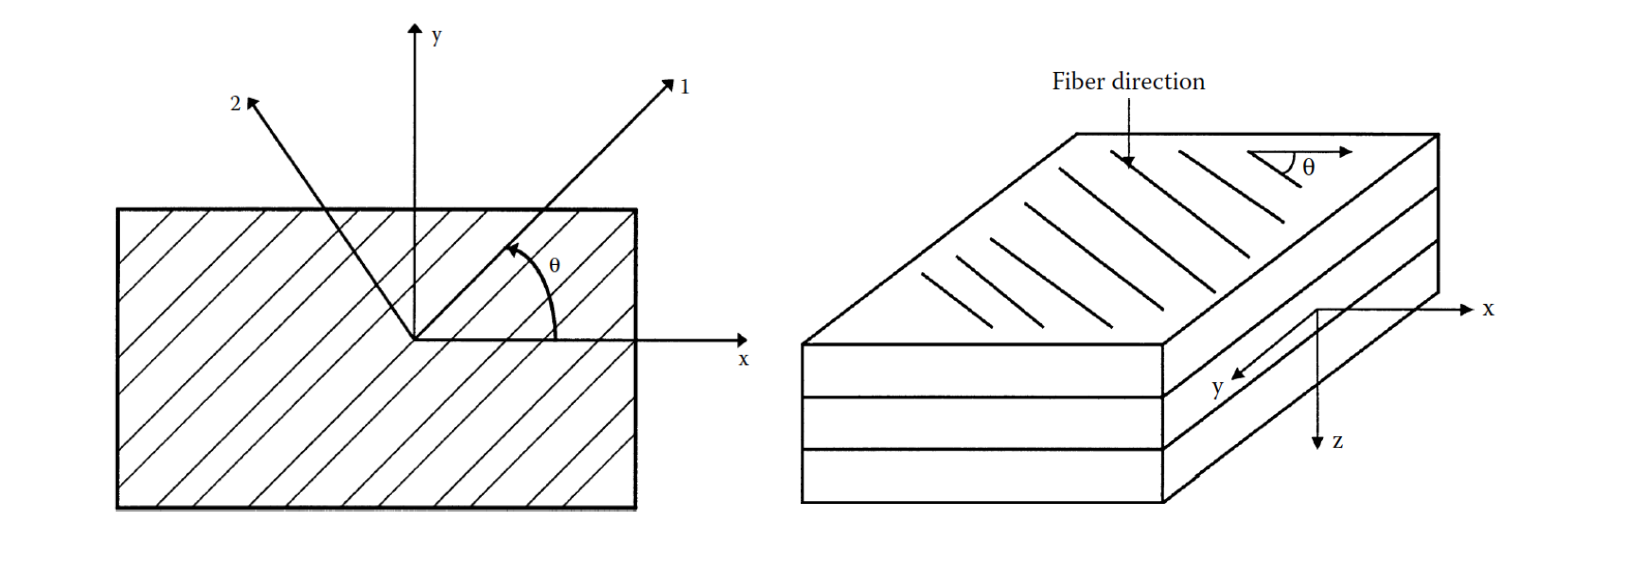
\includegraphics[width=\linewidth]{lamina_local_global_axes.eps}
%\caption{Lamina}
% 	\label{fig:lamina}
%\end{figure*}



\begin{table*}[!htb]
\caption{The optimum lay-ups for the loading $N_x=1e6$ N}
\centering
\begin{adjustbox}{width=1\textwidth}
\begin{tabular}{c|cc|cc}
	\toprule
	Cross Ply $[0_M/90_N]$         & \multicolumn{2}{c}{Previous Research} & \multicolumn{2}{c}{Current Research} \\
	\midrule																								  
	 Material       &  Glass-Epoxy & Graphite-Epoxy  & Glass-Epoxy & Graphite-Epoxy      \\ 
	      M         &  68          &    17           &  78		    &  18             \\
	      N         &  72          &    18           &  28		    &  8              \\
no. of lamina(n)    &  140         &    35           &  106	    &  26                     \\
         SR         &  2.01        &    2.10         &  2.03	    &  2.16            \\
     weight         &  9.10        &    1.84         &  6.89	    &  102.5           \\
	\bottomrule
\end{tabular}
\end{adjustbox}
\label{tab:comparsion}
\end{table*}



The GA process can be divided into two phases by whether there are individuals that are appropriate
or not. During the initial phase, no individual's strength ratio is over the specified threshold, so
individuals with larger fitness are more likely to be chosen as parents, which is why the strength
ratio curves go all the way up to the specified threshold during the first stage. After the initial
phase, the GA produces many appropriate individuals, and then the target function is utilized, and
as shown in Fig. \ref{fig:NxNy}, the fitness curves tend to decrease, but the
strength ratio curves remain greater than the specified threshold.

\begin{table*}[!htb]
\caption{The optimum lay-ups for the loading $N_x=N_y=1e6$ N}
\centering
\begin{adjustbox}{width=1\textwidth}
\begin{tabular}{cccccc}
	\toprule
	 Problem  &    Stacking sequence                                    & Strength ratio  & Mass  &  Cost   & Layer    \\ 
	\midrule																								  
	      I   &  $[\text{-}45_{6}^{cr}/\text{+}45_{6}^{cr}]_s$                        & 2.026           & 1.271 &  192.0  & 24  \\
	      I   &  $[\text{+}45_{10}^{gr}/\text{-}45_{10}^{gr}/\bar{\text{-}45}^{gr}]_s$    & 2.024           & 2.151 &  102.5  & 41  \\
	      I   &  $[\text{-}45_{35}^{gl}/\text{+}45_{36}^{gl}/\bar{\text{+}45}^{gl}]_s$    & 2.001           & 8.980 &  143.0  & 143  \\
	      II  & $[\text{-}45_{9}^{gr}/\text{+}45_{9}^{gr}/\text{-}45_{2}^{cr}/\text{+}45_{2}^{cr}]_s$         & 2.054
										  & 2.313 & 154& 44  \\
	\bottomrule
\end{tabular}
\end{adjustbox}
\label{tab:NxNy}
\end{table*}


In the first experiment, the applied stress is $N_x=N_y=1e6$ N. As shown in
Figure \ref{fig:NxNy}, Figures \ref{fig:NxNy}(a), (b), and (c) show the experimental results for a single material,
Figure \ref{fig:NxNy}(d) shows the results for the hybrid composite material.
 For the single materials, both the basic GA and improved
GA method obtained the optimal value, but the improved GA converged more slowly than the basic GA.
As seen from Table \ref{tab:NxNy}, a $[\text{-}45_{6}/\text{+}45_{6}]_s$ carbon/epoxy
laminate has the least weight, denoted by $W_{min}$, and a
$[\text{-}45_{35}/\text{+}45_{73}/\text{+}45_{35}]$ graphite/epoxy laminate has the lowest cost,
denoted by $C_{min}$. $W_{min}$ and $C_{min}$ were used to evaluate the fitness of the second
problem, which is the layup design of the hybrid composite material. As shown in subfigure d, the
improved GA obtained a more appropriate system layup, whose strength ratio was greater than the
specified safety factor, and the weight and cost are less than the result obtained by the basic GA method, as
shown in Table \ref{tab:NxNy}.
 Compared with the basic GA, the improved GA method showed more powerful
global search ability in the initial phase.

\begin{table*}[!htb]
\caption{The optimum lay-ups for the loading $N_x=N_y=1e6$ N}
\centering
\begin{adjustbox}{width=1\textwidth}
\begin{tabular}{cccccc}
	\toprule
	 Problem  &    Stacking sequence                                    & Strength ratio  & Mass  &  Cost   & Layer    \\ 
	\midrule																								  
	      I   &  $[\text{-}45_{6}^{cr}/\text{+}45_{6}^{cr}]_s$                        & 2.026           & 1.271 &  192.0  & 24  \\
	      I   &  $[\text{+}45_{10}^{gr}/\text{-}45_{10}^{gr}/\bar{\text{-}45}^{gr}]_s$    & 2.024           & 2.151 &  102.5  & 41  \\
	      I   &  $[\text{-}45_{35}^{gl}/\text{+}45_{36}^{gl}/\bar{\text{+}45}^{gl}]_s$    & 2.001           & 8.980 &  143.0  & 143  \\
	      II  & $[\text{-}45_{9}^{gr}/\text{+}45_{9}^{gr}/\text{-}45_{2}^{cr}/\text{+}45_{2}^{cr}]_s$         & 2.054
										  & 2.313 & 154& 44  \\
	\bottomrule
\end{tabular}
\end{adjustbox}
\label{tab:NxNy}
\end{table*}


In the second case, the applied stress was $N_x=N_y=N_z=1e6$ N, and the experimental results were as
shown in the Figure \ref{fig:NxNyNz}. In the first experiment, as seen from Figure \ref{fig:NxNyNz}(a), the improved GA obtained a
better system layup than the result obtained by the basic GA. In the second experiment, as shown in Figure \ref{fig:NxNyNz}(b), during
the initial phase, the fitness curves of the basic GA and improved GA went all the way up to the
previous specified threshold; however, the improved GA converged more slowly than the basic GA, which
means that the search cost of the improved GA was greater than that of the basic GA. After the initial phase, the fitness
curve of the basic GA did not change anymore, it got trapped in the local domain.
 However, the fitness curve of the
improved GA gradually decreased; at the same time, the strength ratio curve of the improved GA
was maintained to be greater than the threshold. This means the improved GA was able to get out of the optimum
and obtain a much better system layup. The improved GA offered more powerful local search
ability. In the third experiment, as shown in Figure \ref{fig:NxNyNz}, both the basic GA and improved
GA obtained the same result, but the improved GA converged more slowly than the basic GA. From these
three experiments for a single material, we know that a $[\text{+}45_{6}^{cr}]_s$ carbon/epoxy laminate has
the least mass, and a $[\text{+}45_{11}^{gl}/\bar{\text{+}45}^{gl}]_s$ glass laminate has the least
cost. In the last experiment, the improved GA obtained a slightly better result than the basic GA,
as shown in Table \ref{tab:NxNyNz}. Compared with the $[\text{+}45_{12}^{cr}]$ laminate, the
weight of a $[\text{+}45_8^{gr}/\bar{\text{+}45}^{gl}]_s$ laminate increased $41.8\%$, however, the
cost decreased $56\%$.
